\section{Apply the privacy-by-design principles using PE-BPMN}

In the previous section we identified unnecessary data leakage risks that result
from improper compliance with privacy-by-design principles. However, before
improving the model by following privacy-by-design principles, we used a tool
called Pleak~\cite{pleaktool} to help verify our findings, and whether we
overlooked additional leakage risks.

Pleak helps with detecting potential privacy risks by identifying sensitive
data, analysing data dependencies and performing differentially private
computations~\cite[311-313]{10.1007/978-3-030-16722-6_18}. The tool can quantify
to what extent a given output leaks information about the input, either in terms
of a sensitivity measure or in terms of the guessing advantage that an attacker
gains by having the output. Additionally, Pleak is a privacy-enhanced extension
of BPMN that enables the modelling of a wide variety of privacy-enhancing
technologies. This enables the analysis of privacy leakage risks and provides a
way to design processes that are more secure and compliant with privacy
regulations~\cite[1-3]{10.1007/s10009-021-00636-w}.

We propose data encryption as a solution for protecting the customer's data from
parties not privy to certain details. The alternatives would have been secret
sharing, data splitting, or a hybrid approach. While the hybrid approach might
offer some more benefits in terms of privacy, using the encryption approach
seemed to be the  most rational in the current case, as there is no handling of
any special type of personal data (like health data, which might require higher
levels of protection). Adding third parties always comes with additional
complexity, which we did not wish to introduce here.

We note that our scheme assumes that a mechanism for key-exchange has been
agreed upon separately, and keys exchanged beforehand, for example, during the
registration flow. The same assumption goes for the license plate information.
We did not add the key-exchange to the model as it is out of scope.

\newpage
The analysis of the model depicted on Figure~\ref{fig:improved-model} provided
the following results:

\begin{center}
\begin{tabular}{ |c||c|c|c|c|c|c|c|c|c|c|c|c|c| } 
    \hline
    & 1 & 2 & 3 & 4 & 5 & 6 & 7 & 8 & 9 & 10 & 11 & 12 & 13\\ 
    \hline
    \hline
    PLT [Processor] & V & - & - & - & V & - & - & V & - & V & V & - & -\\
    \hline
    PSP [Controller] & - & V & V & - & - & V & V & V & - & - & V & V & -\\
    \hline
    User device & - & - & - & O & - & - & - & V & V & - & - & O & -\\
    \hline
    \hline
    Shared over & - & - & - &
    \multicolumn{1}{m{1.2em}|}{MF (V)} &
    \multicolumn{1}{m{1.2em}|}{MF (V)} &
    \multicolumn{1}{m{1.2em}|}{MF (V)} &
    \multicolumn{1}{m{1.2em}|}{MF (V)} &
    \multicolumn{1}{m{1.2em}|}{MF (V)} &
    - & - &
    \multicolumn{1}{m{1.2em}|}{MF (V)} &
    \multicolumn{1}{m{1.2em}|}{MF (V)} & -\\
    \hline
\end{tabular}
\\~\\
V = visible, H = hidden, O = owner, MF = MessageFlow, S = SecureChannel
\end{center}
where the header row numbers represent the following:
\begin{enumerate}
    \item PLTParkingPermitStorage
    \item {[Artifact]} Consent
    \item {[Artifact]} RecordOfProcessing
    \item {[personal\_data]} location
    \item availabilityNotification
    \item location
    \item loginNotification
    \item parkingPermit (PLT name, parking spot, vehicle plate)
    \item parkingPermitStorage
    \item parkingRequest (location)
    \item parkingReservation (location, vehicle plate)
    \item parkingServiceCredential
    \item {[Artifact]} PrivacyPolicy
\end{enumerate}

The results clearly show (e.g., column 6) that the PSP can access the location
of the user and the parking permit, while the PSP does not require access to
those details. Additionally, sensitive data is exchanged without protection. To
mitigate the issues, we complemented our model by implementing data encryption
and secure communication channels. The complemented model is shown on
Figure~\ref{fig:pleak-model}.

\begin{landscape}

\begin{figure}[ht]
\begin{center}
    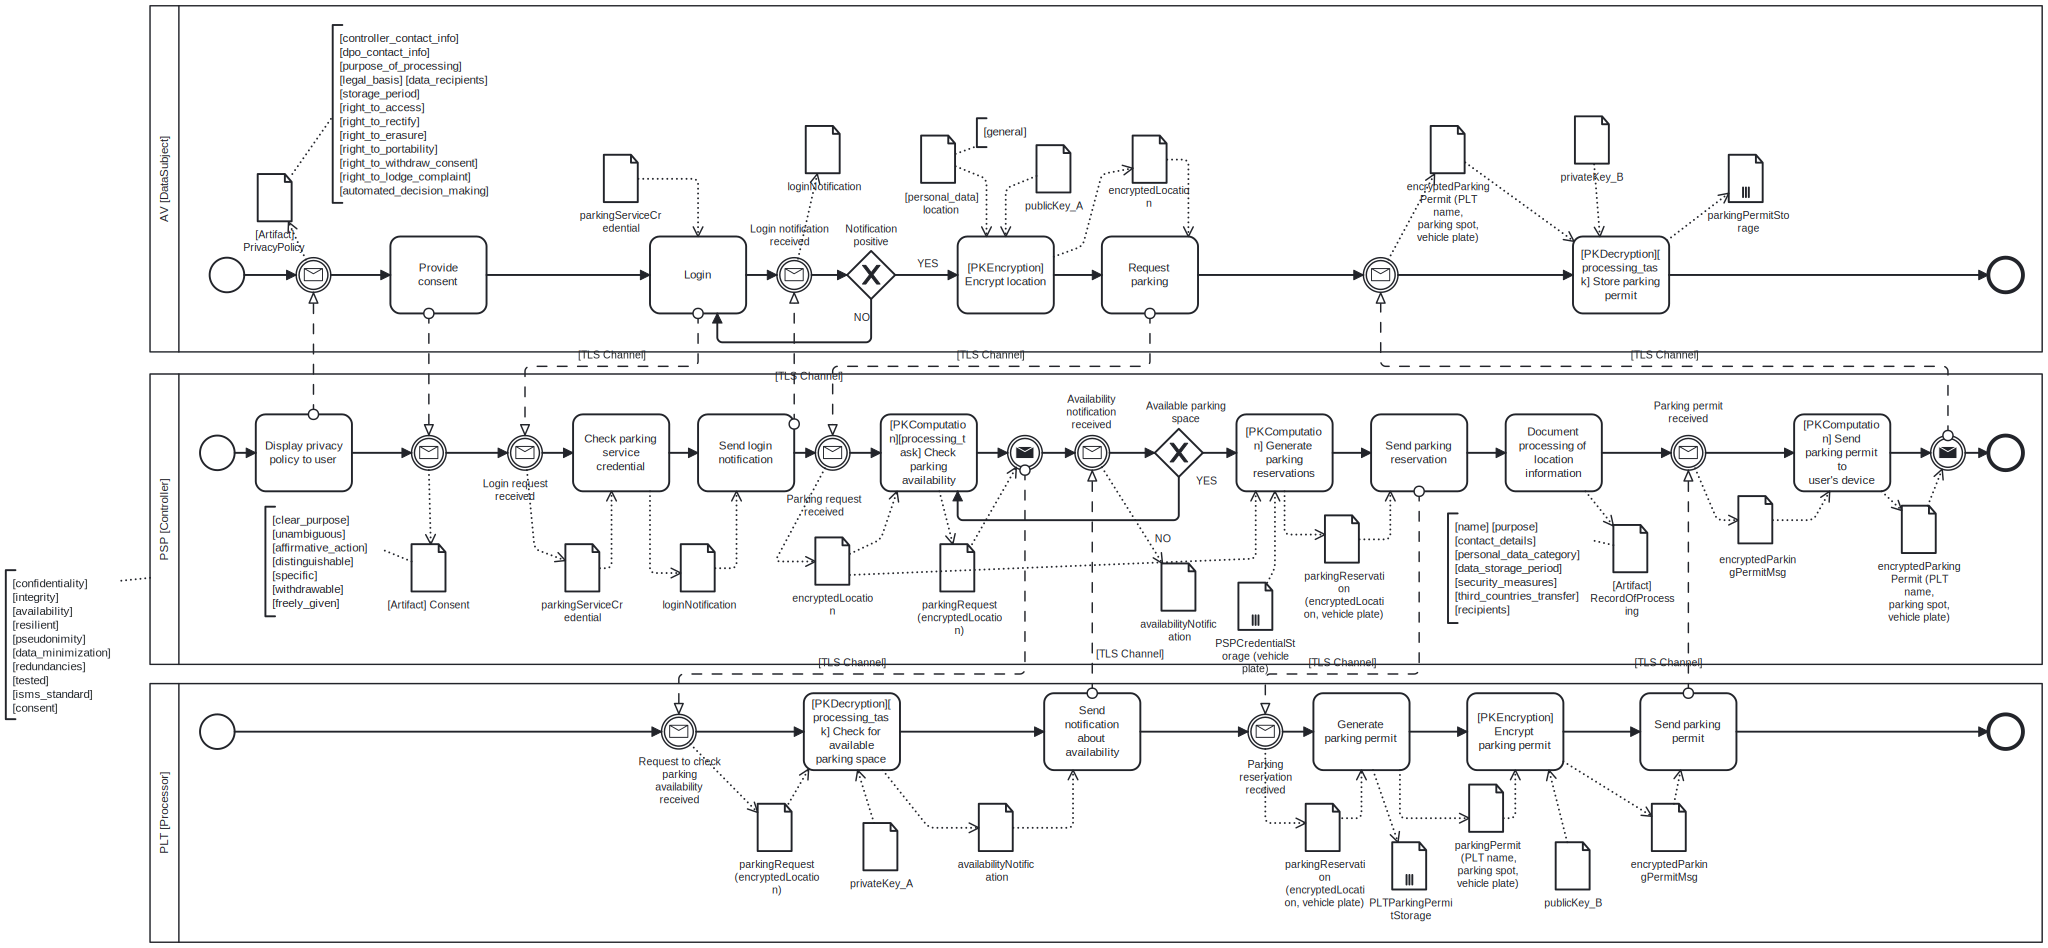
\includegraphics[height=\textwidth - 145pt]{pleak-latest.pdf}
    \caption{PE-BPMN model}
    \label{fig:pleak-model}
\end{center}
\end{figure}

\end{landscape}

The analysis of our complemented model yields the following results:

\vspace{1em} % newline hack
\centerline{
\begin{tabular}{ |c||c|c|c|c|c|c|c|c|c|c|c|c|c|c|c|c| } 
    \hline
    & 1 & 2 & 3 & 4 & 5 & 6 & 7 & 8 & 9 & 10 & 11 & 12 & 13 & 14 & 15 & 16\\ 
    \hline
    \hline
    AV [DataSubject] & - & - & - & V & - & O & V & - & V & - & - & O & - & O &
    O & -\\
    \hline
    PLT [Processor] & V & - & - & - & - & - & - & V & - & V & V & - & O & - &
    - & O\\
    \hline
    PSP [Controller] & - & O & V & - & V & H & V & H & H & V & V & V & - & - &
    - & -\\
    \hline
    \hline
    Shared over & - & - & - & - & - & S & S & S & S & S & S & S & - & - & - &
    -\\
    \hline
\end{tabular}
}
\begin{center}
V = visible, H = hidden, O = owner, MF = MessageFlow, S = SecureChannel
\end{center}
where the header row numbers represent the following:
\begin{enumerate}
    \item PLTParkingPermitStorage
    \item PSPCredentialStorage (vehicle plate)
    \item {[Artifact]} Consent
    \item {[Artifact]} PrivacyPolicy
    \item {[Artifact]} RecordOfProcessing
    \item {[personal\_data]} location, encryptedLocation
    \item loginNotification
    \item encryptedParkingPermitMsg, parkingPermit(PLT name, parking spot,
    vehicle plate)
    \item encryptedParkingPermit (PLT name, parking spot, vehicle plate),
    parkingPermitStorage
    \item availabilityNotification, parkingRequest (encryptedLocation)
    \item parkingReservation (encryptedLocation, vehicle plate)
    \item parkingServiceCredential
    \item privateKey\_A
    \item privateKey\_B
    \item publicKey\_A
    \item publicKey\_B
\end{enumerate}

From the new analysis, we see that some data is now hidden from the PSP, even if
that data is in its possession---sensitive data is now only visible to the
parties requiring it for the purposes of the parking service. By using
encryption, we reduced the risk of data leakage by minimising unnecessary data
access for the PSP without adding much complexity to the overall processes.

In this homework, we identified shortcomings of the initial model regarding GDPR
compliance and data leakage. After identifying the aspects needed to increase
compliance, we complemented the initial model with annotations and additional
actions and used the DPO tool to re-evaluate GDPR compliance. By comparing the
model with privacy-by-design principles, we identified potential data leakage
risks and proposed mitigation strategies stemming from privacy-preserving
technologies. Lastly, we implemented the proposed mitigation strategies into the
model to reduce the leak-surface of the customers' personal data. We also
analysed and validated our improved model with the Pleak tool. Our additions to
the initial model include proper consent management, data processing artifacts,
data encryption, and protected communication between parties.
